%%%%%%%%%%%%%%%%%%%%%%%%%%%%%%%%%%%%%%%
%  Modèle LaTeX pour les documents TB
%
%  Par Charles Duchêne, IG JI
%  Mai 2013
%
%  Toutes les images doivent se trouver
%  dans un sous-dossier pictures
%
%%%%%%%%%%%%%%%%%%%%%%%%%%%%%%%%%%%%%%%

\documentclass[12pt,a4paper]{article}
\usepackage[utf8]{inputenc} 
\usepackage[T1]{fontenc}
\usepackage[pdftex]{hyperref}	
\usepackage{amsmath}
\usepackage{amsfonts}
\usepackage[english,francais]{babel}
\usepackage{telecom}	
\usepackage{aeguill}
\usepackage{times}
\usepackage{listingsutf8}
\usepackage{makeidx}
\usepackage[style=tree,order=word,nonumberlist]{glossaries}
\usepackage{lipsum}
\usepackage{wrapfig}
\usepackage{cite}

%%%%%%%%%%
\usepackage{listings} 			% para llistas de codigo

%%%%%%%%%%%%
\makeindex
\makeglossary

%%%%%%%%%%%%%%%%%%%%%%%%%%%%
% Variables pour ce document
%%%%%%%%%%%%%%%%%%%%%%%%%%%%
\author{Lucas PEREIRA ENDRES}
\title{Developpement d'un multiplexeur MPEG2 compatible avec le standard SBTVD de télévision numérique}
%\contributors{}
\version{1.0}
\docdescription{Stage de Fin d'Études au Brésil \\ \- \\ \textbf{Tuteur:} \\ Altamiro Amadeu SUSIN \\ \textbf{Conseillers d'études:}\\ Michel JEZEQUEL et \\ Sylvie KEROUEDAN\\ 24 février à 25 juillet 2014}
%%%%%%%%%%%%%%%%%%%%%%%%%%%
%%% FICHIER DE CONFIGURATION OPTIONNEL

%%%%%%%% Propriétés pdf %%%%%%%%%%%
\hypersetup{
	bookmarks=true,
	unicode= yes,
	pdftitle={Document témoin du modèle LaTeX pour Télécom Bretagne},
	pdfauthor={Charles Duchêne},
	pdfsubject={},
	pdfkeywords={Télécom, TB, modèle, LaTeX},
	colorlinks=true,
	linkcolor=black,
	citecolor=black,
	filecolor=black,
	urlcolor = black
}

\lstset{
	basicstyle=\ttfamily\small,
	breaklines=true,
	keywordstyle=\bfseries\color{TBbrun},
	inputencoding=utf8/latin1,
}

\lstdefinestyle{stylelatex}{%
	language=tex,
	morekeywords={usepackage,newcommand,begin,renewcommand,section,
	TBannexe,TBsommaire,subsection},
	commentstyle=\itshape\color{TBvert}
}

\lstnewenvironment{latex}{%
	\lstset{style=stylelatex}}{}

\lstnewenvironment{bash}{%
\lstset{
	language=bash,
	basicstyle=\color{white}\ttfamily\small,
	keywordstyle=\color{TBvert}\bfseries,
	backgroundcolor=\color{black},
	morekeywords={sudo, cp, mkdir},
	deletekeywords={local},
}
}{}
 % fichier de configuration optionnel

\lstset{
	basicstyle=\footnotesize\ttfamily,
	%framextopmargin=50pt,
	%frame=lrtb
    language=C,
    frame=single,
    tabsize=2,
    showspaces=false,
    showstringspaces=false,
    keywordstyle=\color{blue},
    %morekeywords={QStringList,QDate,QString,QIODevice},
    commentstyle=\color{CadetBlue},
    %caption={Zistenie, či sme v daný deň, už záznam o rýchlosti uložili},
    breaklines=true
	}

%%%% DÉBUT DOCUMENT
\begin{document}
% ne pas modifier ! imprime la première page du document
\TBfrontcover
\newpage
%%%%%%%%%%%%%%%%%%%%%%%%%%%%
%     CORPS DU DOCUMENT
%%%%%%%%%%%%%%%%%%%%%%%%%%%%
 
\newpage
\section*{Résumé}
La télévision est, parmi les médias de diffusion, le plus important au Brésil. Au début de la dernière décennie, il a été décidé de numériser le système de diffusion de télévision brésilienne. Une action du gouvernement en rejoignant des entreprises et chercheurs de tout le pays a réalisé une étude sur plusieurs sujets de la télévision
numérique. Codage vidéo et audio, ainsi que les sous-systèmes d’interactivité, de multiplexage, de modulation et de transmission sont parmi les aspects étudiés du
système Numérique. Ce qui est ressorti est le SBTVD, le standard de télévision numérique brésilien, qui est basé sur la norme de transmission japonaise, ISDB-T, et
adopte H.264 et HE-AAC comme standards de codage vidéo et audio. Aujourd’hui, la quasi-totalité de l’Amérique du Sud et certains pays africains ont adopté le SBTVD.
L’objectif principal de ce travail est de développer un outil qui crée un flux de transport conforme à la norme brésilienne ABNT NBR15603, à sa fois basée sur la
norme ISO/IEC 13818-1. Pour atteindre cet objectif, une recherche considérable a été réalisée pour comprendre les concepts fondamentaux introduits par ISO/IEC13818-1
et les différences entre cette norme et l’ABNT NBR15603. Certains outils existants génèrent des flux conformes aux normes internationales, mais ne parviennent pas à respecter les spécificités du SBTVD. Une version mise à jour du framework FFmpeg est donc proposée, qui comprend maintenant les structures de données obligatoires
de le SBTVD dans le flux de transport.

%\newpage
\section*{Abstract}
Television is the most important broadcast media in Brazil. At the beginning of the last decade, it was decided to digitize the Brazilian TV broadcast system. A government action joining researchers of all around the country carried out a study on several topics of Digital TV. Video and audio coding, along with interactivity and multiplexing, modulation and transmission subsystems are among the studied aspects of the DTV System. What came out is the SBTVD, the Brazilian DTV standard, which is based on the Japanese ISDB-T transmission standard, and adopts H.264 and HE-AAC as video and audio coding standards. Nowadays, almost all South American and some African countries adopted the SBTVD. The main objective of this work is to develop a tool that creates a Transport Stream compliant to the Brazilian standard ABNT NBR15603 which is based on the ISO/IEC 13818-1 standard. To achieve this objective, considerable research was carried out to understand the fundamental concepts introduced by ISO/IEC13818-1 and the differences between this standard and the ABNT NBR15603. Some existing tools generate streams compliant to the international standards but fail to obey the Brazilian specificities. An updated version of the FFmpeg framework is therefore proposed which now includes the mandatory structures of SBTVD in the Transport Stream.


%% Affichage des listes et tables.
\newpage
\listoffigures  % commenter pour ne pas avoir la liste des figures
\listoftables   % commenter pour ne pas avoir la liste des tables
\newpage
\TBsommaire

\section*{Avertissement / Disclaimer}

\-\newline
Ce travail a été élaboré basé sur la collection de logiciels FFmpeg \cite{ffmpeg} et est soumis à la licence LGPL v2.1 \cite{gplv2}. La partie modifiée du code de FFmpeg est dans la bibliothèque «avformat», qui est le droit d'auteur (C) 2003 de Fabrice Bellard. L'encodeur H.264 utilisé pour créer les échantillons de flux vidéo de ce travail est soumis à la licence GPL et est droit d'auteur (C) 2005 de Rullgard Mans (mans@mansr.com). L'auteur est prêt à aider quiconque soit intéressé à obtenir plus d'informations sur les conditions d'octroi de licences.

\-\newline
This work was developed based on the FFmpeg\cite{ffmpeg} framework and is subject to the LGPL v2.1 Licence \cite{gplv2}. The modified part of FFMpeg code is within the 'avformat' library, which is copyright (C) 2003 of Fabrice Bellard. The H.264 encoder used to create the sample video streams in this work is licenced under the GPL v2 Licence and is copyright (C) 2005 of Mans Rullgard ( mans@mansr.com). The author is willing to help whomever is interested in obtaining further information on licencing conditions.

\-\newline
\begin{minipage}{\linewidth}
\begin{lstlisting}[]
FFmpeg is free software; you can redistribute it and/or modify it under
the terms of the GNU Lesser General Public License as published by the
Free Software Foundation; either version 2.1 of the License,
or(at your option) any later version.

FFmpeg is distributed in the hope that it will be useful, but WITHOUT
ANY WARRANTY; without even the implied warranty of
MERCHANTABILITY or FITNESS FOR A PARTICULAR PURPOSE.
See the GNU Lesser General Public License for more details.

You should receive a copy of the GNU Lesser General Public License
along with FFmpeg; if not, write to the Free Software Foundation, Inc.,
51 Franklin Street, Fifth Floor, Boston, MA 02110-1301 USA.
\end{lstlisting}
\end{minipage}

\-\newline
Les codes sources pour cette modification du code de FFmpeg sont disponibles en Internet sous le système de contrôle de versions Git, à l'addresse suivante:

\-\newline
The source code for this modification is publicly available in the Internet under Git version control system, and may be accessed via the following link:
\begin{verbatim}
https://github.com/nasall2/TCC_ffmpeg
\end{verbatim}

%%%%%% INICIO DO TEXTO PROPRIAMENTE DITO

\newpage
\section{Introduction}

Historiquement, la télévision est présente dans les maisons de la plupart des citoyens brésiliens et elle est la principale source de divertissement et d'information à la population. Au cours des 10 dernières années, les nouveaux médias numériques tels que les téléphones portables et les ordinateurs sont en cours d'adoption par la population de différentes classes sociales. Un rapport récent \cite{pnad2011} dit que, en 2011, 69 \% de la population brésilienne disposait d'une ligne de téléphone mobile. Bien que significative, la participation de ce média reste largement inférieur à celle de la télévision, dont la zone de couverture atteint 100 \% du territoire via satellite \cite{StarOne}, et environ 98 \% de la population par voie terrestre \cite{globo}. La télévision est donc la principale voie de communication à la disposition du grand public au Brésil.

Face aux évolutions des systèmes de codage de médias numériques, permettant de réduire le débit de données pour transmettre de la vidéo de qualité dans les mêmes canaux utilisés pour la télévision analogique, l'ISO e l'IEC ont développé un système de transmission numérique décrit par la norme ISO/IEC13818-1. Commercialement le système est connu sous l'acronyme qui désigne le comité formé pour le rédiger, MPEG2, ou aussi connu comme la recommandation ITU-T H.222. La spécification décrit les standards de codage et transmission de vidéo, audio et des données du système. Une caractéristique clé pour les applications de télévision, c'est qu'il est possible de diffuser des programmes audiovisuels multiples simultanément par un seul diffuseur, dans le même canal physique, permettant ainsi à l'utilisateur de sélectionner les informations qu'il souhaite recevoir parmi plusieurs services envoyés.

Au Brésil, face à l'évolution de la qualité des services de télévision payée à partir de la fin des années 1990, le gouvernement a été poussé à organiser la mise en place du système de télévision numérique terrestre. À cette époque, les opérateurs des chaînes payantes par câble ou par satellite ont débuté les transmissions numériques et il fallait standardiser les transmission numérique via terrestre à fin de faire concurrence aux services payés.

Depuis 1994, les entreprises privées et le gouvernement ont financé de la recherche et des tests techniques à fin de comparer la performance de trois systèmes de télévision numérique qui ont été connus pour être efficaces dans leurs pays d'origine à l'époque: ATSC \cite{ATSC}, développé aux Etats-Unis; DVB-T \cite{DVB}, développé par un consortium d'entreprises et utilisé aux pays européens; et ISDB, développé au Japon par ARIB \cite{ARIB}. Les trois systèmes ont des similitudes et des différences en ce qui concerne l'encodage vidéo et audio: par exemple, DVB et ISDB utilisent l'infrastructure de transport de la norme MPEG2, mais diffèrent dans les schémas de modulation. Après les évaluations, il a été déterminé que le système le plus performant pour le territoire brésilien serait basée sur ISDB, avec quelques modifications, comme indiqué dans le décret présidentiel de création du système\cite{decreto8061}.

Les différences entre l'ISDB original et la norme modifiée utilisée au Brésil concernent principalement l'encodage vidéo et la plate-forme d'interactivité. Afin de promouvoir le développement de l'industrie nationale, le gouvernement a décidé d'adopter une plate-forme open source interactive, nommée Ginga, une technologie développée principalement par des chercheurs brésiliens \cite{PUCRJ}. Grâce à cet outil, le diffuseur peut, par exemple, fournir des informations utiles à la population à faible revenu qui n'a pas d'accès à \textit{Internet}. Une application possible est un projet récemment mis au point, appelé "Brasil 4D" \cite{consultas}. Les utilisateurs peuvent prendre rendez-vous avec des médecins du service public de santé, ou planifier des réunions pour résoudre les problèmes de sécurité sociale, ou bien encore consulter les offres d'emploi en temps réel, tout cela à travers la télécommande du téléviseur. Cependant, la similitude du système brésilien à la norme internationale et le fait que les interfaces interactives ne seront pas obligatoires qu'avant 2015 a conduit à un manque d'intérêt de nombreux diffuseurs dans le développement d'applications, de sorte qu'à l'heure actuelle très peu a été investi dans la création de télévision numérique interactive sur le territoire brésilien.

Le Loi Presidentiel 8061 \cite{decreto8061} du 29 juillet 2013 établit les arrêts progressifs des transmissions analogiques par régions. Jusqu'au 31 décembre 2018, tous les émetteurs analogiques seront désactivés et les canaux doivent être libérées. Les droits d'exploitation des radio-fréquences seront ensuite remis au gouvernement, qui prévoit d'utiliser la bande de 700 MHz pour le service de téléphonie mobile 4G LTE.

Un système de télévision numérique est composé essentiellement par le groupe d'équipements présentés dans la \autoref{fig:diagrama_blocos_tvd}. Au début du flux de signal, il y a des éléments de capture de vidéo et audio, tels que des caméras et des micros. Une fois capturés, la vidéo et l'audio sont compressées et codées par des codeurs correspondants. Le résultat des codeurs sont \textit{bitstreams} standardisés appelés flux élémentaires. Une fois que les flux élémentaires quittent les codeurs, ils entrent dans le multiplexeur, où tous les flux élémentaires sont mis en paquets et intégrés dans un seul flux, appelé flux de transport, ce qui est l'objectif principal de la couche système de MPEG2. Ce qui suit est un processus clé pour la robustesse du système: le flux est protégé par l'emploi de codes de correction d'erreur pour résister au bruit du canal à trajets multiples entre le diffuseur et le récepteur. Enfin, une modulation numérique est appliqué et le flux modulé est envoyé à l'antenne.

 \begin{figure}[!h]
\centering
\caption{Schéma simplifié des flux de signal de la télévision numérique.}
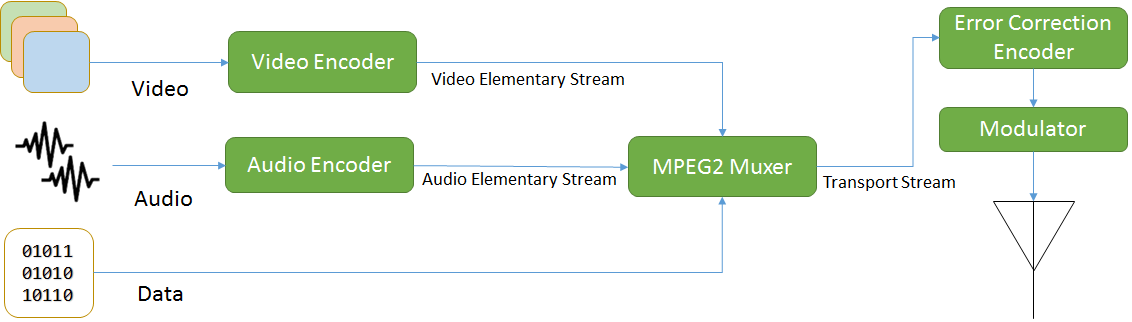
\includegraphics[width=1\linewidth]{pictures/diagrama_blocos_tvd.png}
\label{fig:diagrama_blocos_tvd}
\end{figure}
 
%La principale différence entre les systèmes de télédiffusion analogique et numérique, au niveau de la modulation, est que, dans la télévision analogique le multiplexage est dans le domaine fréquence, le signal vidéo est envoyé dans une bande de fréquence comprise dans la bande passante de canal et le signal audio dans une autre bande de fréquence. Dans la technologie numérique, le multiplexage se passe dans le domaine temporel: la sortie du multiplexeur a un débit constant, et pour les fractions de seconde seulement un paquet d'une des sources de média est envoyé à l'émetteur.

De l'autre côté du canal, le récepteur est conçu de manière à ce que, après passage de la couche de correction d'erreur, un \textit{démultiplexeur} prend le flux composé et le sépare de nouveau dans les flux binaires élémentaires. Ils sont ensuite envoyés aux décodeurs et aux dispositifs de sortie audiovisuels.

Il serait certainement troublant pour le spectateur de regarder les contenus vidéo ou audio en différé, sans synchronisation. Ainsi, un défi de ce schéma de multiplexage est de synchroniser la reproduction de tous les flux de média. Pour ce faire, des labels d'horodatage de présentation sont ajoutés périodiquement dans les flux afin qu'ils puissent être reproduits au même temps.

\section{Objectif et méthodologie}

L'objectif de ce projet est de développer un outil simple, mais flexible, pour gérer la couche des systèmes de la norme SBTVD. Fondamentalement, en utilisant cet outil on est capable de produire un fichier binaire compatible avec le système SBTVD, contenant un flux de transport qui peut être utilisé pour diffuser du contenu audiovisuel  dans des récepteurs appropriés. Beaucoup de solutions commerciales pour cet objectif sont disponibles sur le marché, de sorte que la cible ici n'était pas de développer un produit de consommation, mais plutôt quelque chose de plus académique, éducatif, où la plupart des configurations peuvent être modifiées selon les besoins.

Le client interne principal à l'université (UFRGS) est l'équipe du projet appelé \textit{set-top-box} SBTVD, qui développe un boîtier décodeur du système numérique dans une architecture \textit{System on Chip} sur FPGA. Pour exécuter les tests de l'ensemble du système, les flux de transport avec différentes configurations de multiplexage doivent être diffusées à fin de tester le décodeur sur tous les cas prévus dans la norme.

Le Lapsi (Laboratoire de Traitement du Signal et Images) fait partie du Département d'Ingénierie Électrique (DELET) de l'Université Fédérale du Rio Grande do Sul (UFRGS) et du Programme d'Études Supérieures en Ingénierie Électrique (PPGEE). L'équipe de travail est actuellement composé de cinq enseignants, deux doctorants, 3 masters of science, 3 stagiaires ainsi que et quatre employés, ainsi que la présence d'étudiants exerçant des activités de stages et projets de fin d'études.

Le laboratoire a été créé en 1991 avec l'objectif de combler l'Université dans la recherche au traitement du signal et images. En raison de l'importance atteinte par ces domaines de recherche de nos jours et aux progrès de l'électronique et des télécommunications, le laboratoire fonctionne maintenant aussi dans plusieurs autres domaines de recherche, tels que les tests de systèmes "system-on-chip" (SoC) et projets de la microélectronique analogique et numérique.

%Les créneaux horaires adoptés en concordance avec le superviseur à l'université étaient les suivants: cinq heures par jour les lundis, mercredis et vendredis et trois heures par jour les mardis et jeudis, environ 20 heures par semaine. Cela car en même temps que ce projet a été développé, l'auteur était en cours de stage en entreprise

Le flux de travail du projet a été séparé en trois étapes, selon le descriptif suivant. La première étape a consisté d'une recherche bibliographique à fin d'étudier la norme ABNT NBR15603, ainsi que les références y comprises à la norme ISO/IEC 13818-1 et à la norme ARIB STD-B10. Dans cette étape, l'objectif était de comprendre comment la couche système devrait fonctionner et identifier les composants du multiplexeur qui étaient obligatoires et facultatifs. Une fois que les composants obligatoires étaient connus, les contraintes ont pu être définies. Cependant, si des structures obligatoires sont qu'à titre d'information et son absence ne bloque pas le fonctionnement du système, elles pourraient être laissés au développement futur.

La deuxième étape a envisagé définir le point de départ du développement de l'outil. Aux premières semaines de cette étape, du temps à été consacré à une recherche sur des outils existants aux repositoires d'applications \textit{open-sources} en ligne. Cela a été fait parallèlement à une évaluation de la possibilité de développer l'outil à partir de zéro, parce que d'autres chercheurs dans le laboratoire avaient déjà fait des recherches et avaient conclu que les outils libres trouvées, même avec des modifications, ne pourraient pas gérer les flux selon le standard SBTVD. Au cours de recherches menées par l'auteur lui même, des outils modifiables et avec des fonctionnalités réutilisables ont été identifiés. Ainsi, au lieu de développer à partir de zéro l'outil, il a été décidé de profiter d'un \textit{framework} existant.

Finalement, étant décidé qu'un outil existant serait modifié, la troisième étape a consisté du développement des fonctionnalités manquantes de l'outil choisie de l'étape deux, tout en respectant les contraintes définies à l'étape un, afin de la  rendre compatible avec le SBTVD. Pour valider le projet, les fonctionnalités ont été testés sur différents récepteurs.

L'objectif technique du projet est de fournir un outil qui crée des flux de transport avec trois caractéristiques principales: présentation audiovisuelle synchrone, conformité à la norme SBTVD et possibilité d'envoi de multiples services. Les chapitres que suivent décrivent chacune des étapes citées ci-dessus, en détaillant les démarches suivies et les résultats obtenus.

\section{Norme ISO/IEC 13818-1}
\label{iso13818}

L'objectif principal de la norme ISO/IEC 13818-1 est de décrire la conversion des multiples flux de bits en un seul flux de transport (\textit{Transport Stream}, en anglais, ou TS) enveloppant des données vidéo et audio, ainsi que des informations supplémentaires responsables de déballer les flux de données. De même que d'autres normes ISO/IEC, le texte ne précise que le côté décodage / démultiplexage de la chaîne de transmission, laissant les architectures des étapes de codage / multiplexage à la décision du fabricant.

Certains concepts doivent maintenant être décrits brièvement au lecteur. Le premier est le programme (\textit{program}, en anglais), ou service (homonyme, en anglais), qui est formé par un ensemble d'éléments de programme, qui à leur tour sont appelés flux élémentaires (\textit{elementary streams}, en anglais). Ils peuvent partager une base de temps et donc seront reproduits simultanément. Ceci est équivalent à la notion de chaîne de télévision analogique, dans lequel un diffuseur envoie un flux vidéo et quelques flux audio pour le spectateur. Le second est le \textit{PID}, qui est une étiquette attribuée par la couche système à chaque \textit{payload} transportée dans le TS. Chaque table d'information a son propre PID, chaque flux élémentaire également. Le concept ici est similaire à un pointeur, dans la programmation: lors de la réception d'un paquet TS, le démultiplexeur lit le PID du paquet et pousse sa charge utile au tampon(\textit{buffer}, en anglais) approprié afin que les informations soient  enchaînés avec des paquets précédemment reçus avec la même PID.

La norme définit deux architectures qui doivent être appliqués dans différentes situations. La première consiste à être utilisé dans des situations sans erreur, comme le stockage dans disques numériques, et ne seront plus discutés. L'autre architecture, adaptée aux canaux de transmission susceptibles à erreurs, est appelé le flux de transport. Le paquet du flux de transport a une longueur fixe et est considérablement petit en longueur (188 octets), ce qui le rend facile d'être corrigé par les codes correcteurs d'erreur, afin d'assurer la transmission à travers les canaux défectueux. Des informations plus détaillées peuvent être obtenues dans le rapport complet de projet, en anglais, également disponible.

\subsection{Entête du Transport Stream}
\label{ts_header}

La structure principale du Transport Stream MPEG2 est un paquet de taille constante. Le flux est constitué de paquets concaténés. \autoref{fig:TS_iso13818} montre les éléments qui sont présents dans un paquet, la valeur sous chaque champ est sa longueur en bits. Dans le tableau, on peut voir que le paquet est formé à peu près par 188 octets de données. L'en-tête obligatoire dispose de 4 octets, commence au champs \textit{sync byte} et va jusqu'au \textit{continuity counter}. La charge utile du paquet peut également contenir le \textit{adaptation field}, une sorte d'extension d'en-tête, avec des données supplémentaires qui aident à décoder et à présenter les flux de synchronisation. Outre les 4 octets obligatoires de l'en-tête, les 184 autres octets peuvent être remplis avec une des combinaisons suivantes: le \textit{adaptation field}, les données de PES ou les tables d'information. La présence du champs adaptation field est une option, il est couramment utilisé pour transporter des données de synchronisation et remplir l'espace vide dans le dernier paquet TS transportant un paquet PES avec des bits de bourrage. De plus amples détails sont dans le texte intégral.

\begin{figure}[!h]
\centering
\caption{Formation scheme of a TS packet.}
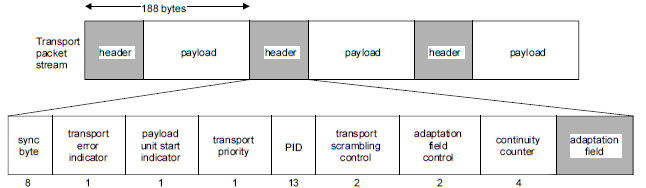
\includegraphics[width=1\linewidth]{pictures/TS_iso13818.png}
\\Source: \cite[F.0.1]{ISO}.
\label{fig:TS_iso13818}
\end{figure}


\subsection{Adaptation Field}

Le \textit{Adaptation Field} (AF) est une extension optionnelle de l'en-tête du paquet TS. Bien qu'il soit facultatif, il contient de nombreuses informations utiles et est largement utilisé dans des applications pratiques pour transporter des informations de synchronisation et de remplir avec des octets de bourrage l'espace vide dans les paquets TS. \autoref{fig:AdapField_iso13818} montre la concaténation des champs du \textit{Adaptation Field}. Une des caractéristiques de cette extension est que beaucoup de champs sont facultatifs, donc il ya plusieurs indicateurs qui font alterner l'existence des champs.

Le champs \textit{adaptation\hspace{0.1mm}\_\hspace{0.1mm}field\hspace{0.1mm}\_\hspace{0.1mm}length} a 8 bits et spécifie le nombre d'octets dans le \textit{Adaptation Field} immédiatement après lui-même. Quand il ya un \textit{payload} partageant le paquet TS avec le \textit{Adaptation Field}, cette valeur doit être dans la gamme 0 à 182. S'il n'y a pas de charge utile, juste le AF, la longueur doit être réglé sur 183. Pour les paquets TS transportant des données du PSE, du bourrage est généralement nécessaire dans le dernier paquet de TS utilisé parce que des paquets PES ne sont pas nécessairement des multiples de 188 octets. Le bourrage est réalisée par réglage de la longueur du \textit{Adaptation Field} de plus que la somme des longueurs des éléments de données, de sorte que les octets de charge utile restantes dans les données PES s'adaptent exactement dans l'espace gauche. L'espace supplémentaire dans le \textit{Adaptation Field} est rempli d'octets de bourrage avec la valeur \texttt{0xFF}.

Le \textit{PCR\hspace{0.1mm}\_\hspace{0.1mm}flag} informe de la présence de l'information optionelle de synchronisation, le PCR, dans les champs \textit{program\hspace{0.1mm}\_\hspace{0.1mm}clock\hspace{0.1mm}\_\hspace{0.1mm}reference\hspace{0.1mm}\_\hspace{0.1mm}base} et \textit{program\hspace{0.1mm}\_\hspace{0.1mm}clock\hspace{0.1mm}\_\hspace{0.1mm}reference\hspace{0.1mm}\_\hspace{0.1mm}extension}. Ces champs sont enveloppés ensemble dans \autoref{fig:AdapField_iso13818} comme «PCR», avec 42 bits. Les autres champs ne seront pas décrits car ils ne sont pas cruciales pour le fonctionnement du multiplexeur. Cependant, ils sont définis dans la norme\cite[2.4.3.5]{ISO}.

\begin{figure}
\centering
\caption{Représentation graphique du  \textit{Adaptation Field}.}
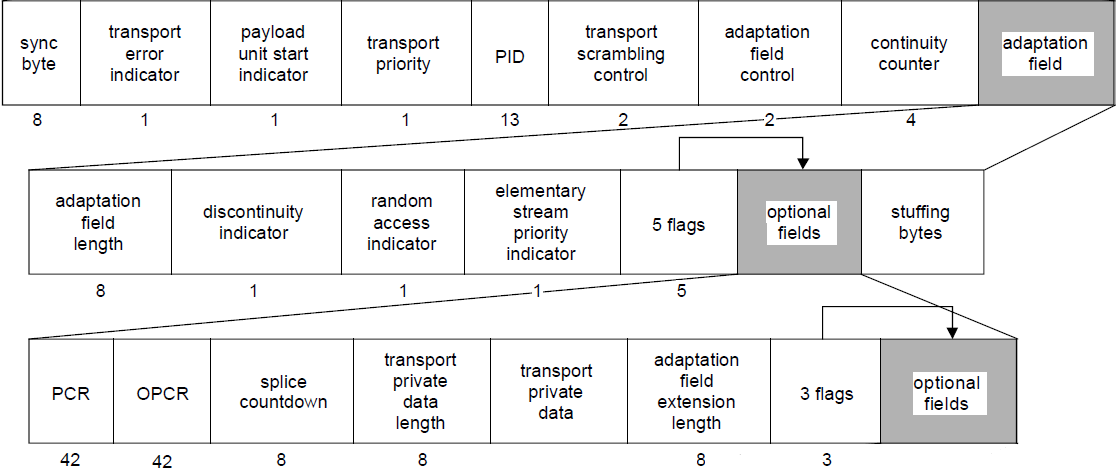
\includegraphics[width=1\linewidth]{pictures/AdapField_iso13818.png}
\\Source et droits d'auteur: \cite[F.0.1]{ISO}.
\label{fig:AdapField_iso13818}
\end{figure}

\subsection{Synchronisation}
\label{Timing}

Les données de vidéo et audio sont transportées par flux séparés qui doivent être reproduites simultanément au niveau du récepteur, de sorte que la synchronisation est crucial pour le fonctionnement d'un système de diffusion de télévision. Le modèle de temporisation introduit par la norme suppose un retard constant de bout en bout à partir de l'entrée du codeur, à travers l'émetteur, le récepteur et jusqu'à à la sortie du décodeur pour tous les flux élémentaires d'un même programme. De cette façon, il est possible d'assurer théoriquement la lecture synchrone de deux flux audio et vidéo.

Le concept clé introduit dans la norme ISO est le \textit{System Time Clock} (STC), une base de temps de référence pour tous les flux dans un même service qui est transmis. L'émetteur contrôle cette référence d'horloge pour les processus et étiquette chaque unité de présentation avec les labels d'horodatage. L'horloge de référence est envoyée par le canal de transmission et le récepteur l'utilise pour verrouiller son propre horloge à la référence. Les trames de média sont transmis avec les labels temporelles, qui sont utilisés par le récepteur pour décoder et présenter les images au moment approprié. 

Si la fréquence du récepteur est la même de l'émetteur, l'encodage, le décodage et taux de présentation seront les mêmes et le système fonctionnera indéfiniment tant qu'il ya des données à transmettre. D'autre part, si les fréquences ne sont pas verrouillés les uns aux autres, une situation de débordement ou soupassement des tampons du décodeur est inévitable et finira par se produire. Si un débordement se produit, les trames seront rejetées et non présentés. Dans le cas de la vidéo encodée avec la prédiction inter-trame, si des trames rejetées seraient utilisés pour décoder d'autres trames, l'ensemble du groupe d'images serait perdu. Si un soupassement se produit, les images seraient figées ou la audio serait muette.

Il est donc important de veiller à la reconstruction de la STC dans le récepteur, car le modèle de retard constant est construit en supposant que les deux parties sont parfaitement en phase et définit les timbres de décodage et de temps de présentation selon la STC. Pour conserver le récepteur verrouillé à l'horloge de référence, une boucle à phase asservie (\textit{phase locked loop}, en anglais) est nécessaire.

\subsection{Program Specific Information}
\label{iso_psi}

\textit{Program Specific Information} (PSI) est un ensemble de données normatives utiles à la transmission, le démultiplexage et la présentation des flux d'audio, de vidéo et de données. L'ensemble du PSI est organisée en tableaux, chacun ayant une fonction spécifique dans la norme. Les tableaux qui transportent l'information sur les PID qui transportent les flux vidéo et audio, appelés PAT (Program Association Table) et PMT (Program Map Table) sont obligatoires et leur syntaxe est définie par la norme ISO/IEC13818-1. La \textit{Network Information Table} est également considérée obligatoire, mais sa syntaxe n'est pas définie par la norme ISO/IEC.

Il y a une autre série de tableaux qui ne sont pas obligatoires selon ISO13818-1, mais la ABNT NBR15603 définit comme obligatoires, comme on le verra dans \autoref{nbr15603}. Bien que l'ISO/IEC13818-1 définit d'autres tableaux, tels que le tableau d'accès conditionnel, ils ne sont pas couramment utilisés en systèmes de radiodiffusion télévisuelle en clair et ont été laissés hors de la portée du projet.

La norme ISO définit que les tableaux PSI doivent être envoyées dans les sections et les sections peuvent être segmentés pour rentrer dans les paquets TS. Les sections ne peuvent pas avoir plus de 1024 octets, mais en pratique, le nombre d'octets pour les tables obligatoires est très en dessous de ce chiffre. Les descripteurs sont des structures utilisées pour étendre les définitions des services et de leurs éléments. Tous les descripteurs ont le même format: ils commencent par une valeur d'étiquette de 8 bits, après il y a un champ de longueur de 8 bits et finalement des octets de données de longueur variable. La norme définit un volume considérable de descripteurs, mais ils ne sont pas tous utilisés dans des applications pratiques.

\section{Norme ABNT NBR15603}
\label{nbr15603}

La norme ABNT NBR15603 est divisé en trois parties, chacune décrit une partie de la couche SBTVD Systems. La plupart du contenu est une adaptation de la norme ISO/IEC13818-1, et il n'y a aucune raison de reproduire ces aspects, mais certaines particularités méritent d'être détaillées. En outre, certaines portions ont été définies sur la base de la norme japonaise ARIB STD-B10. Il existe un ensemble de tableaux obligatoires pour le SBTVD dont la syntaxe n'est pas définie dans les systèmes MPEG-2, notamment le tableau NIT, d'informations du réseau. Les PIDs qui doivent être utilisés pour transmettre les tableaux sont différents de ce qui est défini sur la norme ISO/IEC13818-1 pour quelques tableaux.

\autoref{fig:tab_psi_tables_ids_level_frequency} dans \autoref{tables_abnt} apporte deux autres informations importantes: d'abord, le niveau  de transmission de chaque table, si sa transmission est obligatoire (\textit{"obrigatório"} signifie obligatoire) ou optionnelle; aussi, le taux de répétition de chaque tableau dans le flux, en unités de répétitions par millisecondes. Les tableaux dont la transmission est obligatoire sont la \textit{Program Association Table} (PAT), la \textit{Program Map Table} (PMT), la \textit{Network Information Table} (NIT), la \textit{Service Description Table} (SDT), la \textit{Time Offset Table} (TOT), la \textit{Event Information Table} (EIT) et la \textit{Condition Access Table}  (CAT) (si la transmission est brouillé \footnote{Méthodes de brouillage sont utilisés pour prévenir les récepteurs sans autorisation d'ouvrir certains flux et les afficher. Ils sont généralement utilisés dans les systèmes de télévision payante, mais pas dans les systèmes de diffusion en clair.}).

Les descripteurs sont les structures de données précédemment citées, avec une syntaxe standardisée et qui augmentent la flexibilité des tableaux de porter des informations détaillées sur le système de radiodiffusion, le contenu des flux et les guides de programmation, par exemple. Les longueurs des champs de données sont flexibles, ils dépendent de l'information portée par le descripteur. Si c'est le descripteur du nom du diffuseur, par exemple, il doit être variable, mais si c'est plutôt le descripteur portant la fréquence centrale du canal, il doit toujours avoir la même taille. La norme ABNT définit un ensemble de descripteurs dont la présence est obligatoire dans chacun des tableaux obligatoires.

\section{Available Solutions and Limitations}

Une recherche rapide sur un moteur de recherche pour les mots clés \textit{MPEG2 TS multiplexer} renvoie une longue liste de solutions commerciales ou gratuites pour multiplexer des fichiers médias selon la norme MPEG2.

D'une part, les solutions commerciales sont généralement associées à un matériel dédié, comme la solution présentée par Imagine Communications \cite{harris}. Elles sont ciblés pour les radiodiffuseurs et sont coûteux, de l'ordre de quelques milliers de dollars. Les principaux clients de ces solutions sont les chaînes de télévision, qui transmettent du contenu en direct, et par conséquent le codage du signal et la transmission doivent être à faible latence. Ces appareils fonctionnent en temps réel, en recevant des flux vidéo, audio et de données à travers de multiples interfaces ASI et rendent en sortie un flux multiplexé dans la norme MPEG2.

De l'autre part, les solutions libres sont des logiciels compatibles à la fois avec les plateformes PC Windows et Linux. Certains ont des interfaces graphiques pour aider son utilisation par les utilisateurs peu familiers avec les configurations en ligne de commande, certaines n'ont pas. La principale différence entre les solutions libres et les comerciales est que pour pour celles-ci, la cible n'est pas l'utilisation en temps réel, de sorte que les ordinateurs personnels sont généralement suffisantes pour exécuter les outils. Les interfaces d'entrée et de sortie sont généralement des fichiers qui stockent les flux de données binaires d'une manière séquentielle.

Afin de développer l'outil de multiplexage proposé dans le projet, des outils open-source ont été choisis pour être étudiés. Les critères de choix des solutions sont les suivants:
\begin{itemize}
\item{l'application doit être gratuit et le code source doit être sous licences open-source;}
\item{l'organisation du code source doit faciliter sa modification pour ajouter de nouvelles fonctionnalités et des données;}
\item{l'outil doit être en cours de développement, des solutions sans des mises à jour dans les 5 dernières années n'ont pas été considérés;}
\item{l'outil doit être nativement compatible avec les flux élémentaires définis dans la norme SBTVD, tels que la vidéo H.264 et la audio AAC/LATM.}
\end{itemize}

Une brève description des solutions qui ont atteint la plupart de ces exigences est présentée dans les paragraphes suivants. Après cela, une table synthétise les principales caractéristiques des deux meilleurs d'entre eux.

\subsection{FFMPEG}

Selon les développeurs eux-mêmes, FFmpeg est un outil polyvalent pour le codage, le décodage, la vérification et l'affichage vidéo, audio et de sous-titres. Avec un large ensemble de bibliothèques open source, permet la conversion entre les différents formats, taux de trames, taille d'image vidéo, taux d'échantillonnage audio, entre autres fonctions. Il est le plus complet et soumis à des développements importants, avec des mises à jour quotidiennes organisées dans un dépôt public.

Nativement, il ne permet pas la création de flux TS avec de multiples services (ou programmes). Il est capable de fournir les vidéos en sortie encodées en H.264 et audio encodé en AAC-LATM, comme établit la norme ABNT. Il maintient la synchronisation entre les flux, soit en gardant les informations de synchronisation présents dans les flux d'origine ou en générant de nouvelles références temporelles. Un débit binaire constant du flux TS de sortie peut être réglée et le résultat est fiable.

\subsection{GPAC}

L'outil GPAC a été développé par l'école française Télécom ParisTech, qui a des caractéristiques similaires à FFmpeg, mais est moins performante en garder un chronométrage précis et en maintenir un débit constant du fichier de sortie. Elle prend en charge la création de plusieurs services, mais fait preuve d'un comportement aléatoire du nombre de paquets générés pour les mêmes fichiers d'entrée et les mêmes paramètres de configuration. Par exemple, pour les mêmes fichiers d'entrée avec 10 secondes de durée et les mêmes paramètres d'entrée, l'outil a été testé dix fois et a généré de 7 à 15 secondes de la sortie TS sur dix essais, ce qui suggère un manque de contrôle de débit.

\begin{table}[!htpd]
\caption{Comparaison des Solutions Disponibles}
\begin{center}
\begin{tabular}{|c|c|c|c|}
\hline
Outil & Services Multiples & LATM & Synchronisation\\
\hline
FFmpeg & NON & OUI & OUI\\
\hline
GPAC & OUI & NON & NON\\
\hline
\end{tabular}
\label{tab_comparison_tools}
\\Source: Tests faits par l'auteur.
\end{center}
\end{table}

\subsection{Choix de la Solution}

Même si FFMPEG ne fournit pas de support natif pour les services multiples de la norme MPEG2, il a été choisi comme solution de base pour le projet, car il a été constaté que les modifications apportées au code source afin d'ajouter cette fonctionnalité étaient susceptibles d'être mises en œuvre dans le temps disponible. La fonction de synchronisation existant a favorisé le choix par cette option, aussi. FFMPEG dispose d'une API publique qui aurait pu être utilisé pour développer une application de multiplexage à partir de zéro, mais une modification de la structure existante semblait plus rationnelle compte tenu de l'architecture orientée objet existant et le temps de développement disponible. La plupart des fonctions du multiplexeur MPEG2 existent déjà dans l'ensemble \textit{ffmpeg-formats}, mais il existent des contraintes essentielles au SBTVD qui n'existent pas encore. Les fonctionnalités manquantes, dont le développement est l'objectif de ce projet, sont les suivantes:

\begin{itemize}
\item{ajouter le support aux flux de transport MPEG2 avec services multiples;} 
\item{ajouter les tables qui sont facultatifs dans la norme ISO/IEC, mais sont obligatoires dans le SBTVD.}
\end{itemize}

%%%%%%%
\section{Implementation du Projet}
\label{implementation}

\subsection{Le framework FFmpeg}

Le code source complet de l'application FFmpeg peut être téléchargé gratuitement à partir du site Web du projet \cite{ffmpeg}. Une fois téléchargé, ce que le développeur rencontre est un ensemble de répertoires et de fichiers. Dans le répertoire racine, il y a beaucoup de fichiers texte décrivant en détail les licences, la configuration, la compilation et l'installation de l'outil. FFMPEG est organisé dans la structure suivante: il y a quatre applications exécutables qui résultent de la compilation des paquets et l'installation: \textit{ffmpeg, ffprobe, ffplay} et \textit{ffserver}. Ces quatre applications fonctionnent sur la base de sept bibliothèques qui sont partagées entre les applications, et peuvent également être utilisés à l'extérieur de FFMPEG via une API publique. 

Les bibliothèques gèrent les fonctionnalités de l'outil, qui sont essentiellement l'encodage, le décodage, le filtrage, le multiplexage et le démultiplexage des flux médias. La bibliothèque \textit{libavformat} est responsable des fonctions de multiplexage, et son multiplexeur est compatible avec les contraintes de la ISO/IEC 13818-1. Même si une application peut être développée en utilisant les fonctions de l'API publique, le développement de FFmpeg est fait suivant les concepts de la programmation orientée objet, de manière que les interactions entre les modules sont faciles à comprendre, même pour un lecteur débutant sur le code. Ce qui suit est une description détaillée de l'outil, au niveau du code source. Tout le code est en langage C, sauf indication contraire. Des références pour les notations du langage C utilisés ici sont largement disponibles sur Internet \cite{cpp_reference} ou sur les livres \cite{ritchie}.

%%%%%%%
\section{Tests et Résultats}

\subsection{Environnement de Test}

Le laboratoire dispose de deux systèmes de diffusion de TV: le premier est une station EiTV Playout \cite{eitv}, qui comprend un générateur PSI/SI, un multiplexeur, un modulateur et un émetteur de faible puissance. Il s'agit d'une solution commerciale, qui satisfait aux exigences techniques de la SBTVD mais dont le code source n'est pas ouvert à la contribution. Comme entrées, on fournit un ou plusieurs flux TS, chacun avec un seul service, sous forme de fichiers binaires. Il ne permet pas que les fichiers TS d'entrée contiennent multiples services.

Cette limitation a été une motivation au développement du projet. Ce n'est pas totalement adapté au projet, car il ne permet pas de multiples services dans le même TS d'entrée. Il est utile, d'autre part, pour vérifier la synchronisation des flux audio et vidéo.

L'autre solution disponible est la carte de modulateur PCI Dektec DTA-115, qui est installé dans un poste de travail PC. Ce dispositif est beaucoup plus adapté aux objectifs du projet, parce qu'il reçoit un fichier binaire avec un Transport Stream multi-services et effectue les étapes de modulation et transmission. Sa sortie est un connecteur RF qui est actuellement connecté à une antenne UHF. Une description complète de la carte est disponible dans le site Web du fabricant \cite{dektec}. Le contrôle de la carte se fait en utilisant le logiciel StreamXpress, fourni par le fabricant de la carte.

Deux dispositifs de visualisation sont disponibles pour chaque type de service: un téléviseur LCD Philips et un \textit{set-top-box} EiTV pour la réception full-segment et pour la réception 1-segment un GPS Lenoxx téléphone portable Samsung avec télévision numérique. En outre, un récepteur USB PenTV PixelView reçoit les transmissions Full-segment et 1-segment attaché à un poste de travail Linux. Avec le récepteur USB, les flux de transport sont capturés puis analysés à l'aide de deux logiciels gratuits: \textit{MPEG-2 TS Packet Analyser} et \textit{SBTVD Transport Stream Parser v0.32}. FFprobe est également utilisé comme un outil pour analyser les TS et afficher des informations sur les flux contenus en eux.

\subsection{Tests de Synchronisation}

Ces tests ont été faits avant toute modification dans le code source. L'objectif de ces premiers tests est de vérifier que FFmpeg, snas aucune modification, est capable de fournir un flux de transmission (TS) avec vidéo et audio en synchronisation.

Two different sources of video and audio were tested. The first source is a \textit{mp4} file that contains a video encoded in H.264 with resolution of 720x404 pixels, 23.98 frames per second, and audio encoded in HE-AAC with stereo channels at a sample rate of 48KHz. The second source is another \textit{mp4} file with H.264 video, frame size of 480x360 pixels at 29.97 fps, and stereo HE-AAC audio at 48KHz. The two videos were re-encoded with FFmpeg to output a 1920x1080 frame size at 29,97 frames per second, and the MPEG2 multiplexer was used to create a Transport Stream with one single service. The block diagram in \autoref{fig:test_scn_timing} shows the signal flow.

Deux sources différentes de vidéo et audio ont été testées. La première source est un fichier \textit{mp4} qui contient une vidéo encodée en H.264 avec une résolution de 720x404 pixels, 23,98 trames par seconde, et le dont le son est encodé en HE-AAC avec deux canaux stéréo à un taux d'échantillonnage de 48 kHz. La deuxième source est un autre fichier \textit {mp4} avec de la vidéo H.264, taille d'image de 480x360 pixels à 29,97 images par seconde, et audio stéréo HE-AAC à 48KHz. Les deux vidéos ont été ré-encodées avec FFmpeg pour avoir en sortie une taille d'image de 1920x1080 pixels à 29,97 images par seconde, et le multiplexeur MPEG-2 a été utilisé pour créer un flux de transport avec un seul service. Le schéma fonctionnel dans \autoref{fig:test_scn_timing} montre le flux du signal.

\begin{figure}[!hb]
\centering
\caption{Flux de signal des tests de synchronisation.}
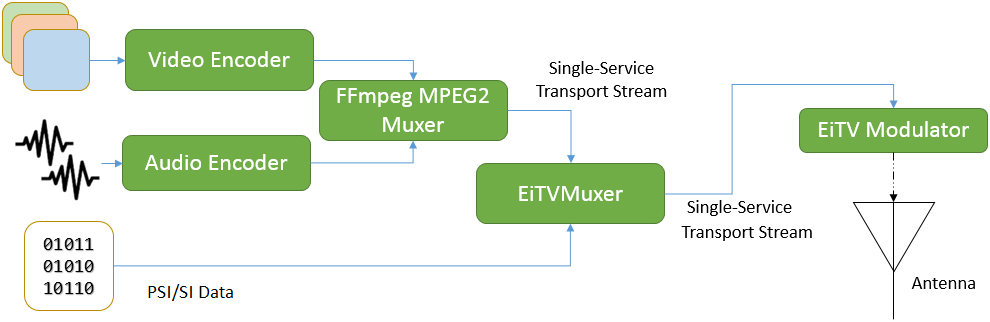
\includegraphics[width=0.9\linewidth]{pictures/test_scn_timing.png}
\\Source: L'auteur.
\label{fig:test_scn_timing}
\end{figure}

% The syntax to call ffmpeg and produce these outputs is shown in \autoref{lst_ffmpeg_single_service}. \texttt{-vcodec libx264 -r 29.97 -s hd1080 -profile:v high} set up the video codec. \texttt{-acodec aac -strict -2 -latm 1} set up the audio codec. \texttt{-t 60} tells the multiplexer to generate a TS with only 60 seconds.

% \begin{minipage}{\linewidth}
% \begin{lstlisting}[caption={Single Service TS creation with FFmpeg.}, label={lst_ffmpeg_single_service}]
% ./ffmpeg -i src.mp4 -vcodec libx264 -r 29.97 -s hd1080 -profile:v high -acodec aac -strict -2 -latm 1 -muxrate 3600000 -t 60 -mpegts_flags latm -loglevel verbose -y dst.ts
% \end{lstlisting}
% \end{minipage}

%Attention should be given to the importance of the \texttt{muxrate} parameter. In the first repetitions of this test, FFmpeg was being called without this option and the output TS ended up with a variable bitrate (VBR), which is not compliant to the MPEG2 standard and leads to a catastrophic loss of sync. When setting up the transmission parameters in EiTV control panel, the TS bitrate must be entered, so the average bitrate of the stream was applied. Since a VBR TS was being broadcast as if it had constant bitrate (CBR), whenever the output bitrate was greater than input bitrate, frames were presented faster than supposed to or skipped. On the opposite case, there were gaps without any frame and the audio would mute or the video would freeze.

Une attention particulière doit être accordée à l'importance de la paramètre \texttt{muxrate}. Dans les premières répétitions de ce test, FFmpeg a été exécute sans cette option et le TS de sortie s'est retrouvé avec un débit binaire variable (VBR), qui n'est pas conforme à la norme MPEG2 et conduit à une perte catastrophique de synchronisation. Si un TS en VBR est diffusé comme s'il avait un débit constant (CBR), chaque fois que le débit de sortie est supérieur à celui de l'entrée, les trames vidéo ou audio sont présentées plus rapidement que le supposé ou sont ignorées. Sur le cas contraire, il y a des moments sans trames dont le son ou la vidéo se figeraient.

%After realizing the need of setting muxrate, it was necessary to know what value should be set. If an underestimated bit-rate is chosen, the PCRs and PTSs will be calculated incorrectly and frames will not be delivered at the expected frame rate. When the transmitter eventually sends the bit-stream to the air in a slower bitrate than necessary, playback will present freeze moments because there will be instants of time without video or audio to be displayed, i.e., it is as if the stream was reproduced in slow motion. On the other hand, an overestimated TS bit-rate causes the multiplexer to add too much stuffing packets into the stream and use unnecessary band.

Après s'être rendu compte de la nécessité de mettre \texttt{muxrate} comme paramètre, il était nécessaire de savoir quel valeur doit être réglée. Si le débit choisi est sous-estimé, les PCR et les PTS seront calculés de manière incorrecte et les cadres ne seront pas présentés à la fréquence attendue. D'autre part, un TS débit binaire surestimé oblige le multiplexeur à ajouter trop de paquets de bourrage dans le flux et utiliser plus de bande que le nécessaire.

%Analyses of the local broadcast channel shown that TSs carried about 11 \% of stuffing bytes, as can be shown in the graphics in \autoref{fig:graph_rbs_dump} and \autoref{fig:graph_band_dump}. The percentages indicated in the figures refer to the amount of data in each PIDs. The PID numbers and packet counts can be seen in \autoref{tab_dumps}. In the graphs, the designation of stuffing packets is \textit{null packet}. From this information, the muxrate option was set at 3.6 Mbps, which results in an overhead of about 11 \%, as can be seen in \autoref{fig:graph_generated_dump}.

Les analyses des flux transmis par les chaînes locales montrent que environ 11 \% des octets transmis sont de bourrage, comme on peut le voir aux graphiques dans \autoref{fig:graph_rbs_dump} et \autoref{fig:graph_band_dump}, dans l'\autoref{resultats}. Les pourcentages indiqués dans les chiffres se rapportent à la quantité de données dans chaque PID. Les numéros de PID et les chiffres de paquets peuvent être vus dans \autoref{tab_dumps}. Dans les graphiques, la désignation des paquets de bourrage est \textit{null packet}. De cette information, l'option \texttt{muxrate} a été fixé à 3,6 Mbps, ce qui se traduit par un bourrage de l'ordre de 11 \%, comme on peut le voir dans l'analyse de l'\autoref{fig:graph_generated_dump}.

% \begin{minipage}{\linewidth}
% \begin{lstlisting}[caption={Output of FFmpeg when input is as \autoref{lst_ffmpeg_single_service}.}, label={lst_ffprobe_clean}]
% Input #0, mpegts, from 'dst.ts':
  % Duration: 00:00:59.98, start: 1.445400, bitrate: 3662 kb/s
  % Program 1 
    % Metadata:
      % service_name    : Service01
      % service_provider: FFmpeg
    % Stream #0:0[0x100]: Video: h264 (High) ([27][0][0][0] / 0x001B), yuv420p, 1920x1080, 29.97 fps, 29.97 tbr, 90k tbn, 59.94 tbc
    % Stream #0:1[0x101](und): Audio: aac_latm ([17][0][0][0] / 0x0011), 48000 Hz, stereo, fltp
% \end{lstlisting}
% \end{minipage}

% FFprobe displays what is in \autoref{lst_ffprobe_clean} when analysing the output of \autoref{lst_ffmpeg_single_service}. The TS lasts 59.98 seconds and has a bitrate of 3662 kbps. It contains only one program, with program\hspace{0.1mm}\_\hspace{0.1mm}number 1, that has two streams: one video stream (PID \texttt{0x100}) and one audio stream (PID \texttt{0x101}) that comply to the requirements of the SBTVD standard.

%The streams were received in the visualization devices and the sync between video and audio was verified by watching and hearing the outputs in scenes where people were filmed while talking. Three different people stated that video and audio were in sync.

%The results were satisfactory, and although there was no employment of functionalities developed by the author, this test was necessary to ensure that the multiplexer could packetize correctly the chunks of data, as well as label the frames with timestamps in sync.

Les flux ont été reçus dans les dispositifs de visualisation et la synchronisation entre la vidéo et l'audio a été vérifiée en regardant et d'entendant les sorties dans les scènes où des personnes ont été filmés tout en parlant. Trois personnes différentes ont déclaré que la vidéo et l'audio sont en synchronisés.

Les résultats ont été satisfaisants, et bien qu'il n'y ait pas d'emploi de fonctionnalités développées par l'auteur, ce test était nécessaire pour s'assurer que le multiplexeur de EiTV pourrait mettre  correctement en paquets les blocs de données, ainsi que d'étiqueter les trames avec des horodateurs.

\subsection{Multiple Services Tests}

%These tests were carried out after applying the implementations described in \autoref{implementation}. Their purpose is to validate the developed system. Two different sets of tests were made, one with a TS captured from a local broadcast channel with the USB receiver and the other with a TS created with the developed multiplexer.

Ces tests ont été réalisés après l'implémentation des fonctionnalités décrites dans \autoref{implementation}. Leur but est de valider le système développé. Deux séries de tests ont été réalisés, l'un avec un TS capturée à partir d'une chaîne locale avec le récepteur USB et l'autre avec un TS créé avec le multiplexeur développé.

\subsubsection{Rétransmission du TS capturé}
\label{retransmitting}

This first set of tests were carried out to understand how the Dektec PCI board works and to validate its functioning. It was done by transmitting a TS that certainly is compliant to the standard, because it was captured from a local broadcaster. The simple block diagram in \autoref{fig:test_scn_retrans} shows the signal flow in this test.

Cette première série de tests a été effectuée afin de comprendre le fonctionnement de la carte PCI Dektec et de valider son fonctionnement. Il a été fait en re-transmettant un TS qui est conforme à la norme, car il a été capturé à partir d'un radiodiffuseur local. Le schéma simplifié de la \autoref{fig:test_scn_retrans} montre le flux du signal dans ce test.

\begin{figure}[!h]
\centering
\caption{Flux de signal des tests de retransmission de TS.}
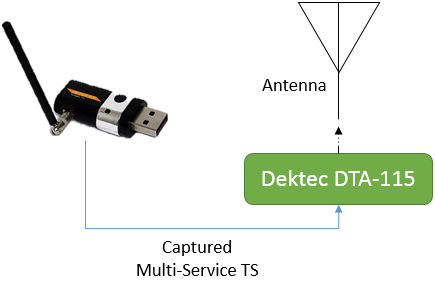
\includegraphics[width=0.5\linewidth]{pictures/test_scn_retrans.png}
\\Source: L'auteur.
\label{fig:test_scn_retrans}
\end{figure}

% The modulator board was configured with the following configuration, which is known to work as informed by previous researchers of the laboratory:

% \begin{itemize}
% \item television broadcast type, mode 3, guard interval 1/16;
% \item partial reception enabled for 1-Segment transmission on layer A;
% \item layer A configured with QPSK modulation, code rate 2/3, time interleave 2 and occupying one segment\footnote{\label{footnote_modulation}Refer to \autoref{modulation}.};
% \item layer B configured with 64QAM modulation, code rate 3/4, time interleave of 2 and occupying twelve segments\footnotemark[\value{footnote}];
% \end{itemize}

With the captured TS file loaded in StreamXpress and these configurations set, in the program interface it is possible to select which PIDs should really be transmitted and in which layer in real-time. Several different combinations of transmitted PIDs and the status of reception in the TV and cell phone are organized in the tables presented in \autoref{resultats}. They are separated by the reception device and within each device separated by its tuning configuration. Several important information can be observed from this tables:
\begin{itemize}
\item all times PAT and NIT were transmitted in layer A, so it can be noticed from \autoref{tab_manual_tuning} that the TV is capable of decoding PIDs sent in the 1-Segment layer;
\item during blind scan, the TV can not find the broadcast channel without the NIT as proved by \autoref{tab_blind_search};
\item in \autoref{tab_normal_operation}, without the PMT, even if the A/V ESs are sent, the TV can not open the streams;
\item the SDT doesn't make difference to the tuning or finding PIDs, but without it the service has no name.
\end{itemize}

With the cell phone, the results are slightly different. There is no manual tuning method, so only blind searches and normal operation tests were done. The results are:

\begin{itemize}
\item from \autoref{tab_cell} it can be seen that PAT presence makes no difference for the phone to open the streams. This is due to the recommendation on NBR 15608, for 1-Segment PMTs to have a default PID range;
\item without NIT, the phone can not find the broadcast channel in blind search. If NIT is removed after blind search, the phone keeps receiving as long as PMT is still being sent.
\end{itemize}

This whole set of tests provides now information about what to expect when the stream generated by the developed multiplexer is broadcasted.

\subsubsection{Transmitting a remultiplexed TS with two services}
\label{test_remultiplexing}

The main objective of this last set of tests is to confirm that the developed multiplexer creates a TS compliant to the standard and that it is received and decoded correctly. The two inputs are edited Transport Streams which were captured and remultiplexed, one contains the Full Segment service and the other, the 1-Segment service. The signal flow is shown in \autoref{fig:test_scn_muxing}

\begin{figure}[!h]
\centering
\caption{Signal flow for remultiplexed TS tests.}
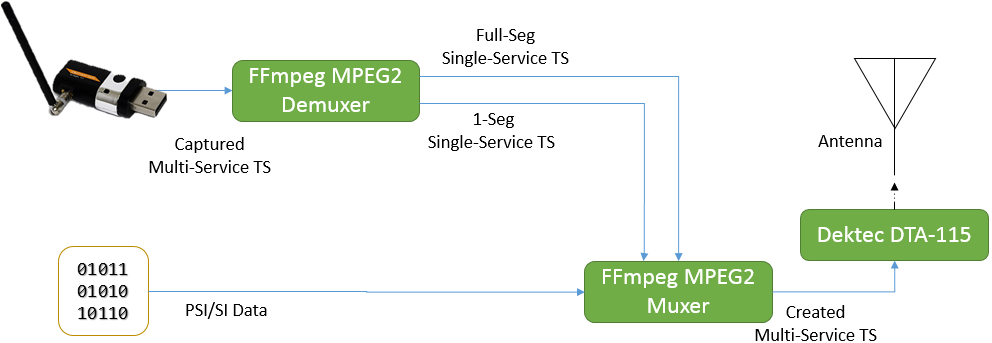
\includegraphics[width=0.8\linewidth]{pictures/test_scn_muxing.png}
\\Source: The author.
\label{fig:test_scn_muxing}
\end{figure}

The TS was generated using the following configurations, which are compliant to the standard: the physical network characteristics are original network ID 0730, area code 2970, guard interval 1/16, transmission mode 3, physical channel 20 and virtual channel 1. The transmission profile is set as 1. \autoref{lst_ffmpeg_multi_service} shows the command-line call and \autoref{lst_ffprobe_multi_service} shows the FFprobe analysis results.

\begin{minipage}{\linewidth}
\begin{lstlisting}[caption={FFmpeg command-line call to generate a multi-service TS}, label={lst_ffmpeg_multi_service}]
./ffmpeg -i /var/src/tve_HD_0406.ts -i /var/src/tve_LD_0406.ts -map 0:0 -map 1:0 -map 0:1 -map 1:1 -vcodec copy -acodec copy -mpegts_original_network_id 0730 -mpegts_area_code 2970 -mpegts_guard_interval 2 -mpegts_transmission_mode 3 -mpegts_physical_channel 20 -mpegts_virtual_channel 1 -mpegts_transmission_profile 1 -muxrate 12000000 -mpegts_flags latm -loglevel verbose -t 30 -y /home/nethome/endres/TVE_HD_LD.ts
\end{lstlisting}
\end{minipage}

\begin{minipage}{\linewidth}
\begin{lstlisting}[caption={FFprobe analysing the multi-service TS.}, label={lst_ffprobe_multi_service}]
Input #0, mpegts, from '/home/nethome/endres/TVE_HD_LD_long_1406.ts':
  Duration: 00:01:01.36, start: 1.400000, bitrate: 11972 kb/s
  Program 23360 
    Metadata:
      service_name    : SVC HD Full Seg
      service_provider: FFmpeg
    Stream #0:0[0x100]: Video: h264 (High) ([27][0][0][0] / 0x001B), yuv420p(tv, bt709), 1920x1080 [SAR 1:1 DAR 16:9], 29.97 fps, 29.97 tbr, 90k tbn, 59.94 tbc
    Stream #0:1[0x102](por): Audio: aac_latm ([17][0][0][0] / 0x0011), 48000 Hz, stereo, fltp
  Program 23385 
    Metadata:
      service_name    : SVC LD 1-Seg
      service_provider: FFmpeg
    Stream #0:2[0x101]: Video: h264 (Constrained Baseline) ([27][0][0][0] / 0x001B), yuv420p, 320x240 [SAR 1:1 DAR 4:3], 14.99 fps, 29.97 tbr, 90k tbn, 29.97 tbc
    Stream #0:3[0x103]: Audio: aac_latm ([17][0][0][0] / 0x0011), 48000 Hz, stereo, fltp
\end{lstlisting}
\end{minipage}

\begin{figure}[!h]
\centering
\caption{TS Parser output for four different Transport Streams.}
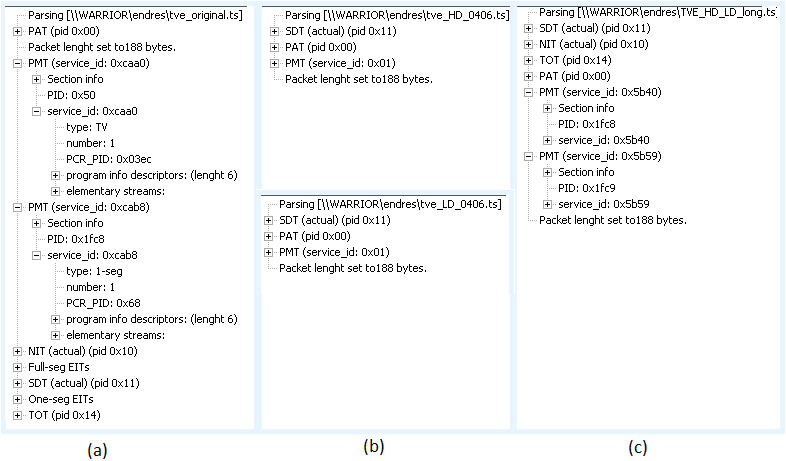
\includegraphics[width=0.9\linewidth]{pictures/ts_parser_tve_orig_remux.png}
\\Source: The author.
\label{fig:ts_parser_tve_orig_remux}
\end{figure}

\autoref{fig:ts_parser_tve_orig_remux} shows the output of MPEG2 Parser for the original captured TS in (a), the two streams derived from it in (b) and the remultiplexed TS by this project in (c). In (a), one may notice the presence of all PSI/SI tables. In (b), only one PMT remains on each edited TS and since they were generated with the original FFmpeg, SI tables are not present(NIT, TOT), except the SDT\footnote{An SDT without all the required information is generated by FFmpeg automatically.}. In (c), the PSI/SI tables are recreated with the developed solution and the service numbers are no longer the same, since network characteristics are different from the original captured TS.

In \autoref{fig:ts_parser_tve_remux_pmt} the TS Parser is analysing the PMTs of the remultiplexed TS. In the left side is the PMT for Full-Segment service, where service ID \texttt{0x5B40} can be identified, the parental rating descriptor is indicating that the show if free for all ages in Brazil and the Elementary Streams described are one video of type H.264 at PID \texttt{0x100} (the primary video ES) and one AAC/LATM audio of PID \texttt{0x102}. The parser lacks the syntax of some descriptors and can not show the AAC descriptor, for example, but it can be seen that its tag is \texttt{0x7C} and content is \texttt{0x2E} as indicated by \autoref{pmt_descriptors}.

In the right side of \autoref{fig:ts_parser_tve_remux_pmt}, the same as above is valid, but the video stream is identified as 1-segment primary video and the service number is \texttt{0x5B59}.

It is interesting to show here that the stream mapping explained in \autoref{stream_mapping} actually worked. The first input stream was the HD video and it received the PID \texttt{0x100}. The second was the 1-Segment video, assigned PID \texttt{0x101}. The third was HD audio, that got PID \texttt{0x102}, and 1-Segment audio got PID \texttt{0x103}.

\begin{figure}[!h]
\centering
\caption{TS Parser analysing PMTs of remultiplexed TS.}
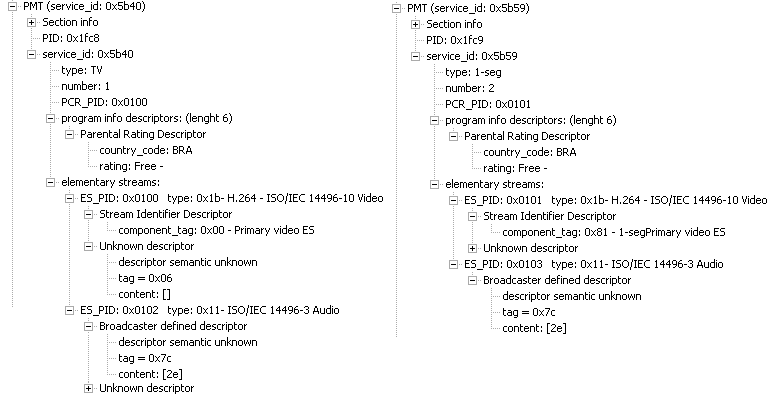
\includegraphics[width=0.9\linewidth]{pictures/ts_parser_tve_remux_pmt.png}
\\Source: The author.
\label{fig:ts_parser_tve_remux_pmt}
\end{figure}

In \autoref{fig:ts_parser_tve_remux_nit} the TS Parser is analysing the NIT of the remultiplexed TS. Since the table is too long, it was split in two parts as shown by the arrow. From the network descriptors tree, it is seen that the default network name was used in the Network Name Descriptor. The parser lacks the syntax of the System Management Descriptor. Further in the tree, one sees the value ZYA730 as the Original Network ID, the value that was passed as a parameter to FFmpeg.

Within the TS descriptors, the TS name holds the same name of the network, as defined by the SBTVD standard. In the Transmission loop, the two services have their modulation schemes detailed, as well as the service types, numbers and IDs. In the rightmost part of \autoref{fig:ts_parser_tve_remux_nit}, the Partial Reception Descriptor points that service \texttt{0x5B59} is for 1-Segment reception. Finally, the Terrestrial System Delivery Descriptor carries many of the options passed to FFmpeg, all according to the expected.

\begin{figure}[!h]
\centering
\caption{TS Parser analysing NIT of remultiplexed TS.}
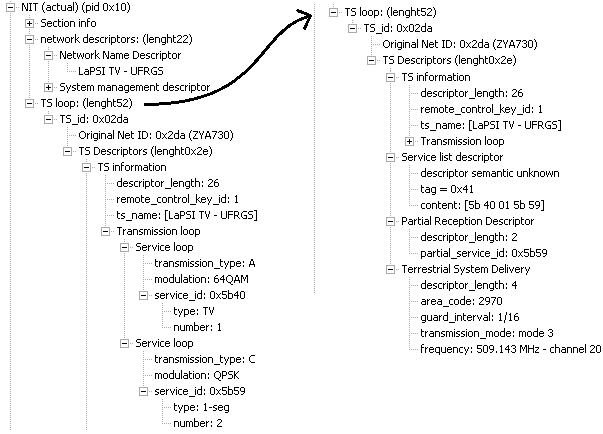
\includegraphics[width=0.9\linewidth]{pictures/ts_parser_tve_remux_nit.png}
\\Source: The author.
\label{fig:ts_parser_tve_remux_nit}
\end{figure}

In \autoref{fig:ts_parser_tve_remux_sdt} the TS Parser is analysing the SDT of the remultiplexed TS. Once again the service IDs and service types are shown, as well as the EIT scheduling flags indicating that there is neither EPG information nor EIT tables. The Service Descriptors show the service names, providers and service types.

\begin{figure}[!h]
\centering
\caption{TS Parser analysing SDT of remultiplexed TS.}
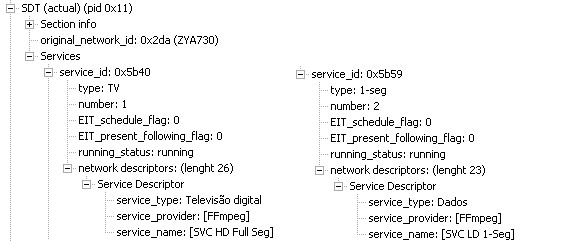
\includegraphics[width=0.9\linewidth]{pictures/ts_parser_tve_remux_sdt.png}
\\Source: The author.
\label{fig:ts_parser_tve_remux_sdt}
\end{figure}

After this complete analysis among the PSI/SI tables generated by the code developed in the project, it can be seen that all the transmitted tables and descriptors are compliant to the standard and contain valid information. Also, the information in the tables is readable by the receptors as will be seen next. The EIT table and its descriptors, not yet implemented, did not block the system functionalities. The TOT table is currently presenting errors in operation and although it was generated, it was not broadcasted.

The same sequence of tests of \autoref{retransmitting} was carried out for this Transport Stream. The results were similar as in the other tests, which is why the tables with results are not presented. Instead, some pictures were taken to illustrate the system working.

\autoref{fig:video_audio_both} shows a scene with a dB meter close to the TV speaker. In the left picture are being transmitted PAT, PMTs, NIT, SDT and video ES, but no audio ES; the audio level is 61dB. In the right picture the audio ES is sent along with the other PIDs and the level increases (to 71dB), as expected.

In \autoref{fig:info_with_without_sdt} it can be seen the effect of sending the SDT into the Transport Stream. In the left side, there is PAT, PMT, NIT but no SDT, and therefore there is no name next to the virtual channel number. In the right, on the other hand, the SDT is sent and the name "SVC HD Full Seg" is shown, which is the default name configured by the C macros in FFmpeg, as expected.

In the left side of \autoref{fig:cell_with_sdt}, the reception on the cell phone can be seen. Overlapped to the video is the channel list with the selected virtual channel '1' and the network name describing the channel. In the right side, a manual tuning is being performed in the channel 20 of the TV and no ESs nor the SDT are being sent, only PAT, PMTs and NIT. It can be seen that the channel name is empty but there is a "good" reception level. The "Channels found" flag indicates that PAT and PMT for the HD service are present, but the blue screen points that there is no ESs to be decoded.

%%%%%%%
\section[Conclusions and Future Development]{Conclusions and Future Development}

La télévision est le média de communication le plus répandu au Brésil, les émissions terrestres couvrent jusqu'à 70 \% de la population et les gens comptent sur la télévision pour satisfaire leurs besoins d'information et de divertissement. En outre, les systèmes de télévision payés offrent une vidéo de haute qualité et du contenu audio haute définition, et les abonnements deviennent moins chers chaque année. Il existe un risque important que, sans la migration des transmissions de télévision analogique terrestres vers un système numérique de haute qualité, les diffuseurs vont perdre leur audience à la télévision payé. Il est techniquement impossible de diffuser des programmes de télévision multiples ou augmenter la qualité des médias dans les canaux analogiques existants. Il est donc nécessaire d'adopter un système de transmission numérique, à fin de fournir la solution aux problèmes techniques et commerciaux soulignés.

Après des années de discussions, le consortium brésilien a décidé de baser son système de télévision numérique, le SBTVD-T, sur celui fait par les Japonais, le ISDB-T. Les aspects techniques qui ont conduit à ce choix à la place des autres étaient la faible consommation d'énergie grâce à l'amélioration des schémas de modulation et la possibilité de diffuser vers les appareils mobiles ainsi que des dispositifs fixes dans le même canal physique.

La motivation de cette étude est née de la nécessité d'un outil pour tester la \textit{set-top box} qui est développé dans le Laboratoire de traitement des signaux de l'Université. Il n'y avait pas d'outil disponible pour multiplexer et diffuser les flux élémentaires de référence, nécessaires pour tester la réception et le décodage de l'appareil. Par conséquent, l'objectif du projet était de développer un outil flexible et gratuit qui permet la transmission de flux multimédia selon la norme brésilienne.

Pour atteindre cet objectif, il était nécessaire d'étudier les normes ISO/IEC13818-1 et NBR15603. Après des recherches pour des solutions similaires qui existaient déjà, FFmpeg a été jugée très facilement modifiable, et a été choisi comme point de départ du développement. Comme méthodes pour valider la mise au point, un ensemble de quatre récepteurs ont été utilisés, ainsi que des outils pour analyser les fichiers de binaires générés.

Bien que le code de FFmpeg était abondamment commenté, la manque de documentation de l'outil a conduit à plusieurs erreurs aux premiers tests. Par exemple, il n'y avait aucune indication de l'unité de mesure de l'option \textit{muxrate} et il a été supposé comme «kbps» d'abord. Après des flux générés à tort, on s'est rendu compte que l'unité a été plutôt «bps». En outre, le \textit{flag} LATM dans le multiplexeur n'active pas vraiment l'encapsulation du flux audio en LATM, mais il ne définit que la valeur d'un champs dans le descripteur de flux du tableau PMT. Ceci a été découvert après n'avoir pas de réception audio dans le récepteur set-top-box EiTV alors qu'il y avait dans le récepteur audio Philips TV. Cela est probablement dû au fait que le téléviseur est équipé aussi d'un décodeur audio compatible aux normes de télévision numérique autres que SBTVD, et ainsi reçoit du contenu hors les contraintes de la norme.

En plus des tests qui ont été déjà réalisées, des expérimentations supplémentaires peuvent être faites en appliquant des images vidéo de référence à l'entrée du multiplexeur. L'état de développement actuel le permet. De plus, les étapes de codage et de multiplexage des flux qui sont faites séparément peuvent être combinés en une seule étape, de sorte que la même entrée vidéo puisse générer des services à la fois la HD et 1-segment.

En reprenant les objectifs définis au chapitre d'introduction, on peut voir que les tâches proposées ont toutes été accomplies. Le projet fournit un outil qui est conforme à la norme SBTVD, transmet la vidéo et l'audio en synchronisation et permet la diffusion de multiples services. La conformité de FFmpeg à la norme SBTVD et le support des flux à services multiples sont les deux fonctionnalités ajoutées par ce projet. Les fonctionnalités de synchronisation existaient déjà, bien que personne dans le laboratoire aurait pu consacrer suffisamment d'efforts pour la faire fonctionner avant.

La conformité à la norme SBTVD a été obtenue en ajoutant les tables d'information de système qui n'étaient pas présentes dans le logiciel de FFmpeg originel. Le \textit{Network Information Table} (NIT) est crée correctement, vu que les récepteurs sont capables d'identifier l'existence du canal transmis en leur présence. Sans envoyer le tableau, cependant, la chaîne n'est pas identifié. Le \textit{Service Description Table} (SDT) est également correcte, comme les récepteurs parviennent à montrer les noms de service quand ils reçoivent ce tableau.

Les analyses effectuées sur les flux générés montrent la formation de presque tous les descripteurs, les exceptions sont ceux dont les analyseurs n'arrivent pas à décoder. Tous les descripteurs de programmes et du système ajoutés sont interprétées correctement par TS Analyser et TS Parser, comme l'a montré les tests décrits dans les chapitres précédents.

La conformité avec le SBTVD n'est pas encore mis en œuvre, cependant. Même si il a été prouvé que le flux multiplexé peut être reçu par les dispositifs et ils parviennent à le décoder correctement, le \textit{Event Information Table} (EIT), qui est obligatoire, n'est pas encore implémentée. Ce tableau n'est pas responsable du réglage du tuner, de la démodulation, ni du décodage, il est purement informative et c'est pour cela qu'il a été laissé à la poursuite du développement. Le système fonctionne sans lui.

Par ailleurs, le \textit{Time Offset Table} (TOT) et son descripteur obligatoire ont bien été mis en œuvre, mais quand ils ont été transmises l'information de la date et de l'heure dans les récepteurs n'a pas été mise à jour comme indiqué dans le tableau tous les temps. Pas beaucoup de temps a été consacré jusqu'à maintenant à comprendre pourquoi cette question arrive, parce que le multiplexeur fonctionne sans cette information. Il n'existe aucune relation entre l'affichage de l'heure et la présentation des flux en synchronisation.

Surtout, les parties qui ne sont pas encore mises en œuvre sont décrites dans les chapitres théoriques et peuvent être développés avec peu d'effort, à l'aide de l'architecture FFmpeg et en profitant de certains des algorithmes décrits par l'auteur.

Le développement futur de ce projet peut être fait pour tourner l'interface de l'outil plus convivial. Il est intéressant de créer une interface utilisateur graphique avec des listes de valeurs valides des paramètres et l'état du processus de multiplexage. En outre, une caractéristique clé encore à mettre en œuvre est le deuxième profil de transmission, qui permettra la création de flux de transport avec plus que deux services. Le profil 2 est déjà défini et décrit dans le texte, et des extraits de code peuvent être réutilisés pour mettre en œuvre cette fonctionnalité.

% ANNEXES
\appendix
\newpage
\TBannexe{Tableaux et Images des Résultats des Tests}
\label{resultats}

\begin{figure}[!h]
\centering
\caption{Packets distribution among PIDs in local broadcaster A.}
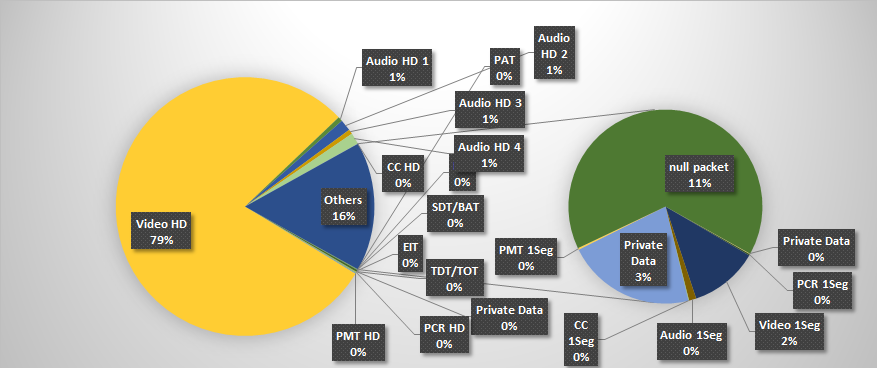
\includegraphics[width=0.9\linewidth]{pictures/graph_rbs_dump.png}
\\Source: The author.
\label{fig:graph_rbs_dump}
\end{figure}

\begin{figure}[!h]
\centering
\caption{Packets distribution among PIDs in local broadcaster B.}
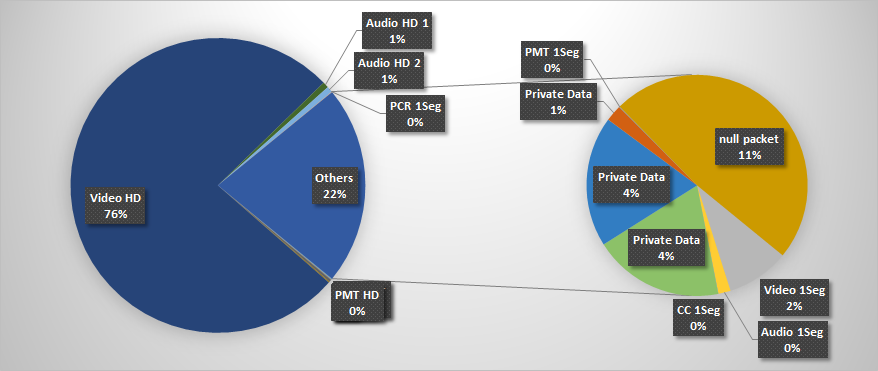
\includegraphics[width=0.9\linewidth]{pictures/graph_band_dump.png}
\\Source: The author.
\label{fig:graph_band_dump}
\end{figure}

\begin{table}[b]
\centering
    \caption {Data from stream aquisitions.}
    \begin{tabular}{|l|l|l|l|l|l|l|}
    \hline
     Bcaster A  & Bcaster A          & Bcaster A    & ~ & Bcaster B & Bcaster B         & Bcaster B   \\ \hline
    PID   & Type         & Count  & ~ & PID  & Type         & Count  \\ \hline
    0     & PAT          & 260    & ~ & 0    & PAT          & 100    \\ \hline
    16    & NIT          & 26     & ~ & 16   & NIT          & 10     \\ \hline
    17    & SDT/BAT      & 13     & ~ & 17   & SDT/BAT      & 5      \\ \hline
    18    & EIT          & 734    & ~ & 18   & EIT          & 10     \\ \hline
    20    & TDT/TOT      & 5      & ~ & 20   & TDT/TOT      & 2      \\ \hline
    39    & Private Data & 115    & ~ & 36   & ~            & 10     \\ \hline
    256   & PCR HD       & 452    & ~ & 39   & ~            & 10     \\ \hline
    257   & PMT HD       & 261    & ~ & 233  & CC HD        & 27     \\ \hline
    273   & Video HD     & 237551 & ~ & 256  & PCR HD       & 264    \\ \hline
    274   & Audio HD 1   & 1729   & ~ & 257  & PMT HD       & 100    \\ \hline
    275   & Audio HD 2   & 4288   & ~ & 273  & Video HD     & 76284  \\ \hline
    276   & Audio HD 3   & 1745   & ~ & 274  & Audio HD 1   & 654    \\ \hline
    277   & Audio HD 4   & 4280   & ~ & 275  & Audio HD 2   & 660    \\ \hline
    278   & CC HD        & 53     & ~ & 512  & PCR 1Seg     & 47     \\ \hline
    500   & Private Data & 51     & ~ & 529  & Video 1Seg   & 2006   \\ \hline
    512   & PCR 1Seg     & 114    & ~ & 530  & Audio 1Seg   & 394    \\ \hline
    529   & Video 1Seg   & 5551   & ~ & 549  & CC 1Seg      & 4      \\ \hline
    530   & Audio 1Seg   & 585    & ~ & 1000 & Private Data & 4169   \\ \hline
    534   & CC 1Seg      & 53     & ~ & 1001 & Private Data & 4168   \\ \hline
    900   & Private Data & 10415  & ~ & 4101 & Private Data & 521    \\ \hline
    8136  & PMT 1Seg     & 132    & ~ & 8136 & PMT 1Seg     & 26     \\ \hline
    8191  & null packet  & 31587  & ~ & 8191 & null packet  & 10529  \\ \hline
    Total & ~            & 300000 & ~ & ~    & ~            & 100000 \\ \hline
    \end{tabular}
	\label{tab_dumps}
\end{table}

\begin{figure}[!h]
\centering
\caption{Packets distribution among PIDs in generated TS.}
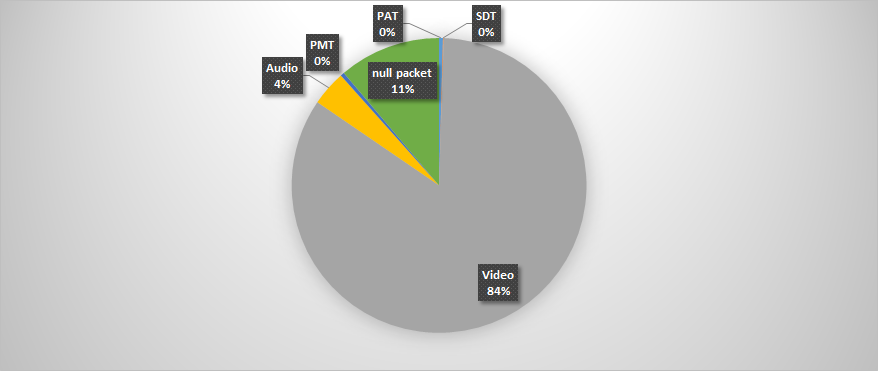
\includegraphics[width=0.9\linewidth]{pictures/graph_generated_dump.png}
\\Source: The author.
\label{fig:graph_generated_dump}
\end{figure}

\begin{table}
    \caption {Cell phone in blind search and normal operation.}
    \begin{center}
\begin{tabular}{|l|l|l|}
    \hline
    Sent PIDs              & Finds channel in blind search & Status in normal operation \\ \hline
    NIT                    & YES                           & "Signal too weak, retry?"  \\ \hline
    PAT, PMT, SDT, A/V ESs & NO                            & Opens A/V                  \\ \hline
    NIT, PMT, SDT, A/V ESs & YES                           & Opens A/V                  \\ \hline
    NIT, PMT, A/V ESs      & YES                           & Opens A/V                  \\ \hline
    \end{tabular}
	\label{tab_cell}
\end{center}
\end{table}

\begin{table}
    \caption {TV receiver in manual tuning method.}
    \begin{center}
\begin{tabular}{|l|l|l|l|}
    \hline
    Sent PIDs                   & Signal Level & Screen / Speakers Status & Service Name \\ \hline
    NIT                         & 0            & Blue Screen              & NONE         \\ \hline
    NIT, PAT                    & Good         & Blue Screen              & NONE         \\ \hline
    NIT, PAT, PMT               & Good         & Blue Screen              & NONE         \\ \hline
    NIT, PAT, PMT, A/V ESs      & Good         & Video and Audio in Sync  & NONE         \\ \hline
    NIT, PAT, PMT, A/V ESs, SDT & Good         & Video and Audio in Sync  & HDTV SVC \\ \hline
    \end{tabular}
	\label{tab_manual_tuning}
\end{center}
\end{table}

\begin{table}
    \caption {TV receiver in normal operation mode.}
    \begin{center}
\begin{tabular}{|l|l|l|l|}
    \hline
    Sent PIDs               & Opens A/V & "No Signal" & "No available \\
                   & Streams & Flag & programme" flag \\ \hline
    NIT                     & NO                & YES              & NO                            \\ \hline
    NIT, PAT                & NO                & NO               & YES                           \\ \hline
    NIT, PAT, PMT           & NO                & NO               & YES                           \\ \hline
    NIT, PAT, PMT, Video ES & YES, video only   & NO               & NO                            \\ \hline
    NIT, PAT, A/V ESs  & NO         & NO               & YES                            \\ \hline
	NIT, PAT, PMT, A/V ESs  & YES, both         & NO               & NO                            \\ \hline
    \end{tabular}
	\label{tab_normal_operation}
\end{center}
\end{table}

\begin{table}
    \caption {TV receiver in blind search mode.}
    \begin{center}
\begin{tabular}{|l|l|}
    \hline
    Sent PIDs & Finds channel \\ \hline
    NIT       & YES           \\ \hline
    PAT, PMT  & NO            \\ \hline
    PAT       & NO            \\ \hline
    NIT, PAT  & YES           \\ \hline
    \end{tabular}
	\label{tab_blind_search}
\end{center}
\end{table}

\begin{figure}[!h]
\centering
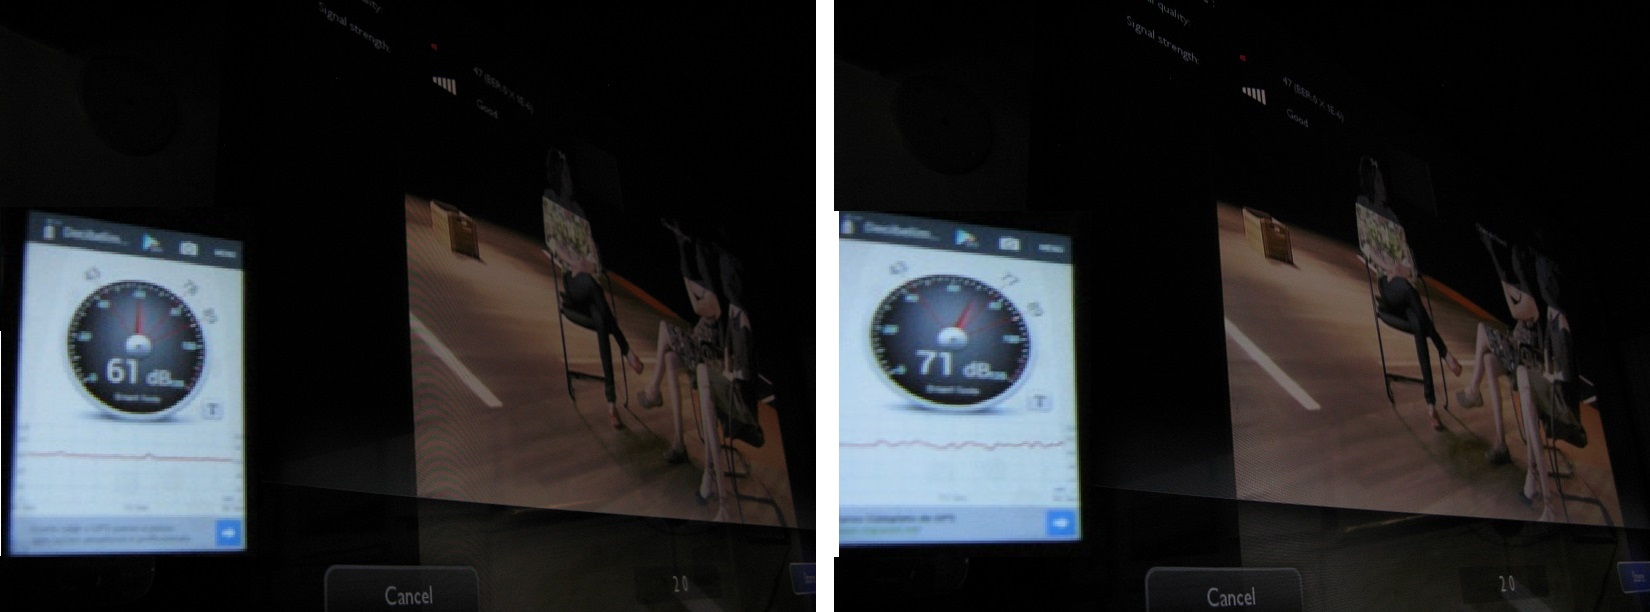
\includegraphics[width=0.9\linewidth]{pictures/video_audio_both.jpg}
\\Source: The author.
\caption{Reception of video with and without audio.}
\label{fig:video_audio_both}
\end{figure}

\begin{figure}[!h]
\centering
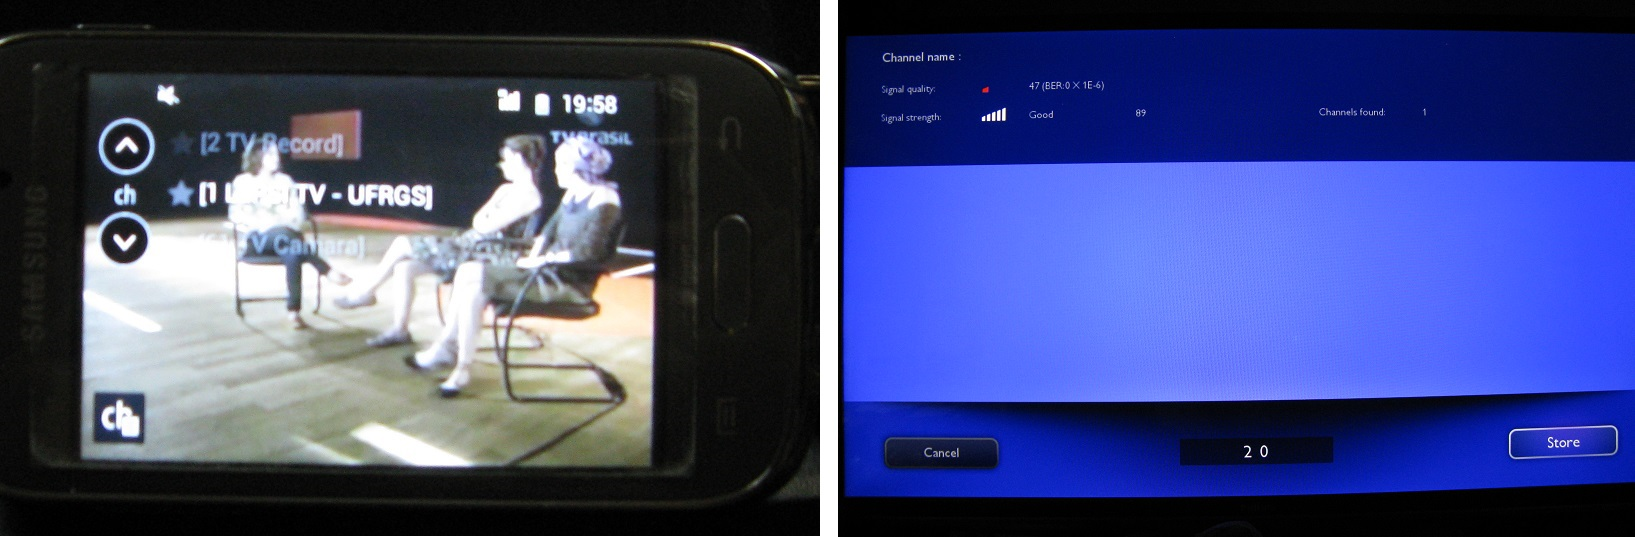
\includegraphics[width=0.9\linewidth]{pictures/cell_with_sdt.jpg}
\\Source: The author.
\caption{Reception in the Cell Phone and TV manual tuning.}
\label{fig:cell_with_sdt}
\end{figure}

\begin{figure}[!h]
\centering
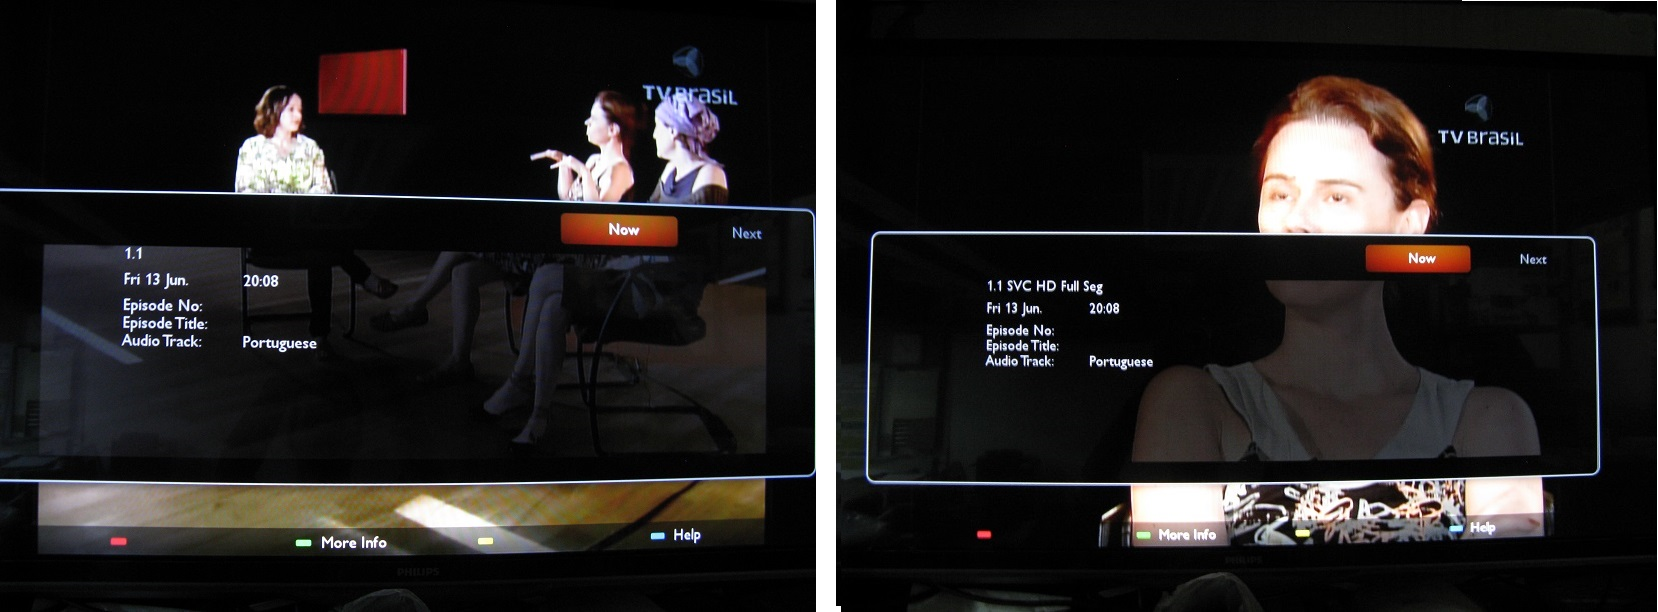
\includegraphics[width=0.9\linewidth]{pictures/info_with_without_sdt.jpg}
\\Source: The author.
\caption{Service information with and without SDT.}
\label{fig:info_with_without_sdt}
\end{figure}

\newpage
\TBannexe{Aspects du système de transmission du SBTVD}
\label{modulation}

Dans le ISDB-T, un canal UHF est divisée en 13 segments de fréquence. Les récepteurs à bande étroite sont capables de décoder uniquement la fréquence(ou segment)  centrale du canal, qui sont communément appelés des récepteurs 1-segment. Les récepteurs à large bande, qui peuvent décoder tous les 13 segments de fréquence, sont appelés décodeurs full segment. \autoref{fig:ISDB-T_CH_Seg_Prog_allocation} montre la répartition des segments à l'intérieur d'un canal. «S0» est le segment central pour les tuners à bande étroite. «S1» à «S12» sont les autres segments.

Le plus la bande est étroite, le plus petite est la quantité d'informations qui peuvent être envoyées à travers elle. Les récepteurs 1-segment sont utilisés dans les appareils mobiles, et sont capables de recevoir des vidéos de basse définition (basse qualité) uniquement, avec un seul flux audio. Les récepteurs full-segment sont utilisés dans des dispositifs fixes, tels que les téléviseurs Full-HD, et sont capables de décoder la vidéo haute définition avec plusieurs flux audio.

Les schémas de modulation habituellement utilisés dans «S0» sont différents de ceux des autres segments. Comme les transmissions de TV 1-segment ciblent les appareils mobiles, la portée du signal doit être plus élevé et au plus une petite antenne dipôle est disponible au récepteur, alors une modulation QPSK est utilisée. Pour les autres segments, la quantité de données est beaucoup plus élevé, et aux clients il ne les dérange pas d'avoir une antenne amplifiée attaché à l'arrière de leur téléviseur, de sorte qu'une modulation moins robuste est appliquée, comme 64QAM.

\begin{figure}[!h]
\centering
\caption{Canal ISDB-T et ces segments.}
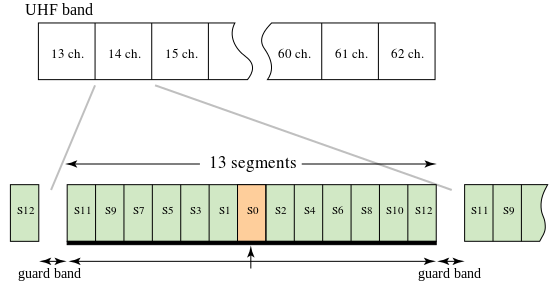
\includegraphics[width=0.8\linewidth]{pictures/ISDB-T_CH_Seg_Prog_allocation.png}
\\ Source: UnLiM, derivé de Namazu-tron, obtenu en Wikipedia \cite{ISDB_wiki}
\\ Licensed under Creative Commons 3.0 via Wikimedia Commons
\label{fig:ISDB-T_CH_Seg_Prog_allocation}
\end{figure}

%%%%%%%%%%%

%\section{Tests}
%\newpage
%\TBannexe{}
%\section{123}
%\subsection{222}
%\subsection{444}



% INDEX, RÉFÉRENCES et GLOSSAIRE
\newpage
\-\-\-
\newpage
\TBindex
\TBbiblio{plain-fr}{includes/biblio}
\TBglossary

% ne pas modifier ! imprime la dernière page du document
\TBcoverpage
\end{document}
